\documentclass{beamer}
\usepackage{graphicx}
\usepackage{epstopdf}
\usepackage{hyperref}
\usecolortheme{seagull}

\title{Cognitive Radio Test-Bed using OpenBTS}
\author{Swrangsar Basumatary (09d07040)}
\institute{Department of Electrical Engineering \\ IIT Bombay, Powai}
\date{June 2014}

\setbeamertemplate{frametitle}[default][center]
\setbeamerfont{frametitle}{size=\Large,series=\bfseries}
    
\begin{document}
  \frame{\titlepage}


	\begin{frame}{Problem Statement}
    	\begin{itemize}
    		\item To develop a test-bed for cognitive radio demonstrating coexistence of primary (licensed) users and secondary (unlicensed users)
    		\item A 2-frequency test-bed (channels used 945 MHz and 955 MHz)
    		\item A 4-frequency test-bed (936 MHz, 943 MHz, 950 MHz, 957 MHz)
    	\end{itemize}
	\end{frame}
	
	\begin{frame}{Overview of the tasks accomplished in our project}
		\begin{itemize}
      \item Cognitive radio?,  spectrum holes?
      \item GNURadio
      \item Python programming language
      \item USRP kit
      \item OpenBTS
      \item Calls and SMS service on local network
      \item Spectrum sensing techniques
      \item Defining problem statement
    \end{itemize}
  \end{frame}
    
    \begin{frame}{}
        \begin{itemize}
		\item Developing a flow chart of the solution to this problem
		\item Running GNURadio and OpenBTS  on the same computer at the same time
		\item Bash scripting ( .sh files)
		\item Periodogram analysis
		\item Building a 2-frequency cognitive radio test bed
		\item Building a 4-frequency cognitive radio test bed
		\end{itemize}
	\end{frame}
	
	\begin{frame}{Hardware and software used}
    \begin{itemize}
      \item GNURadio
      \item OpenBTS
      \item USRP N210  Kits
      \item GSM mobile phones with SIM cards
      \item Computers
    \end{itemize}
  \end{frame}

  \begin{frame}{Setup for the 2-frequency test-bed}
    \begin{figure}
      \centering
      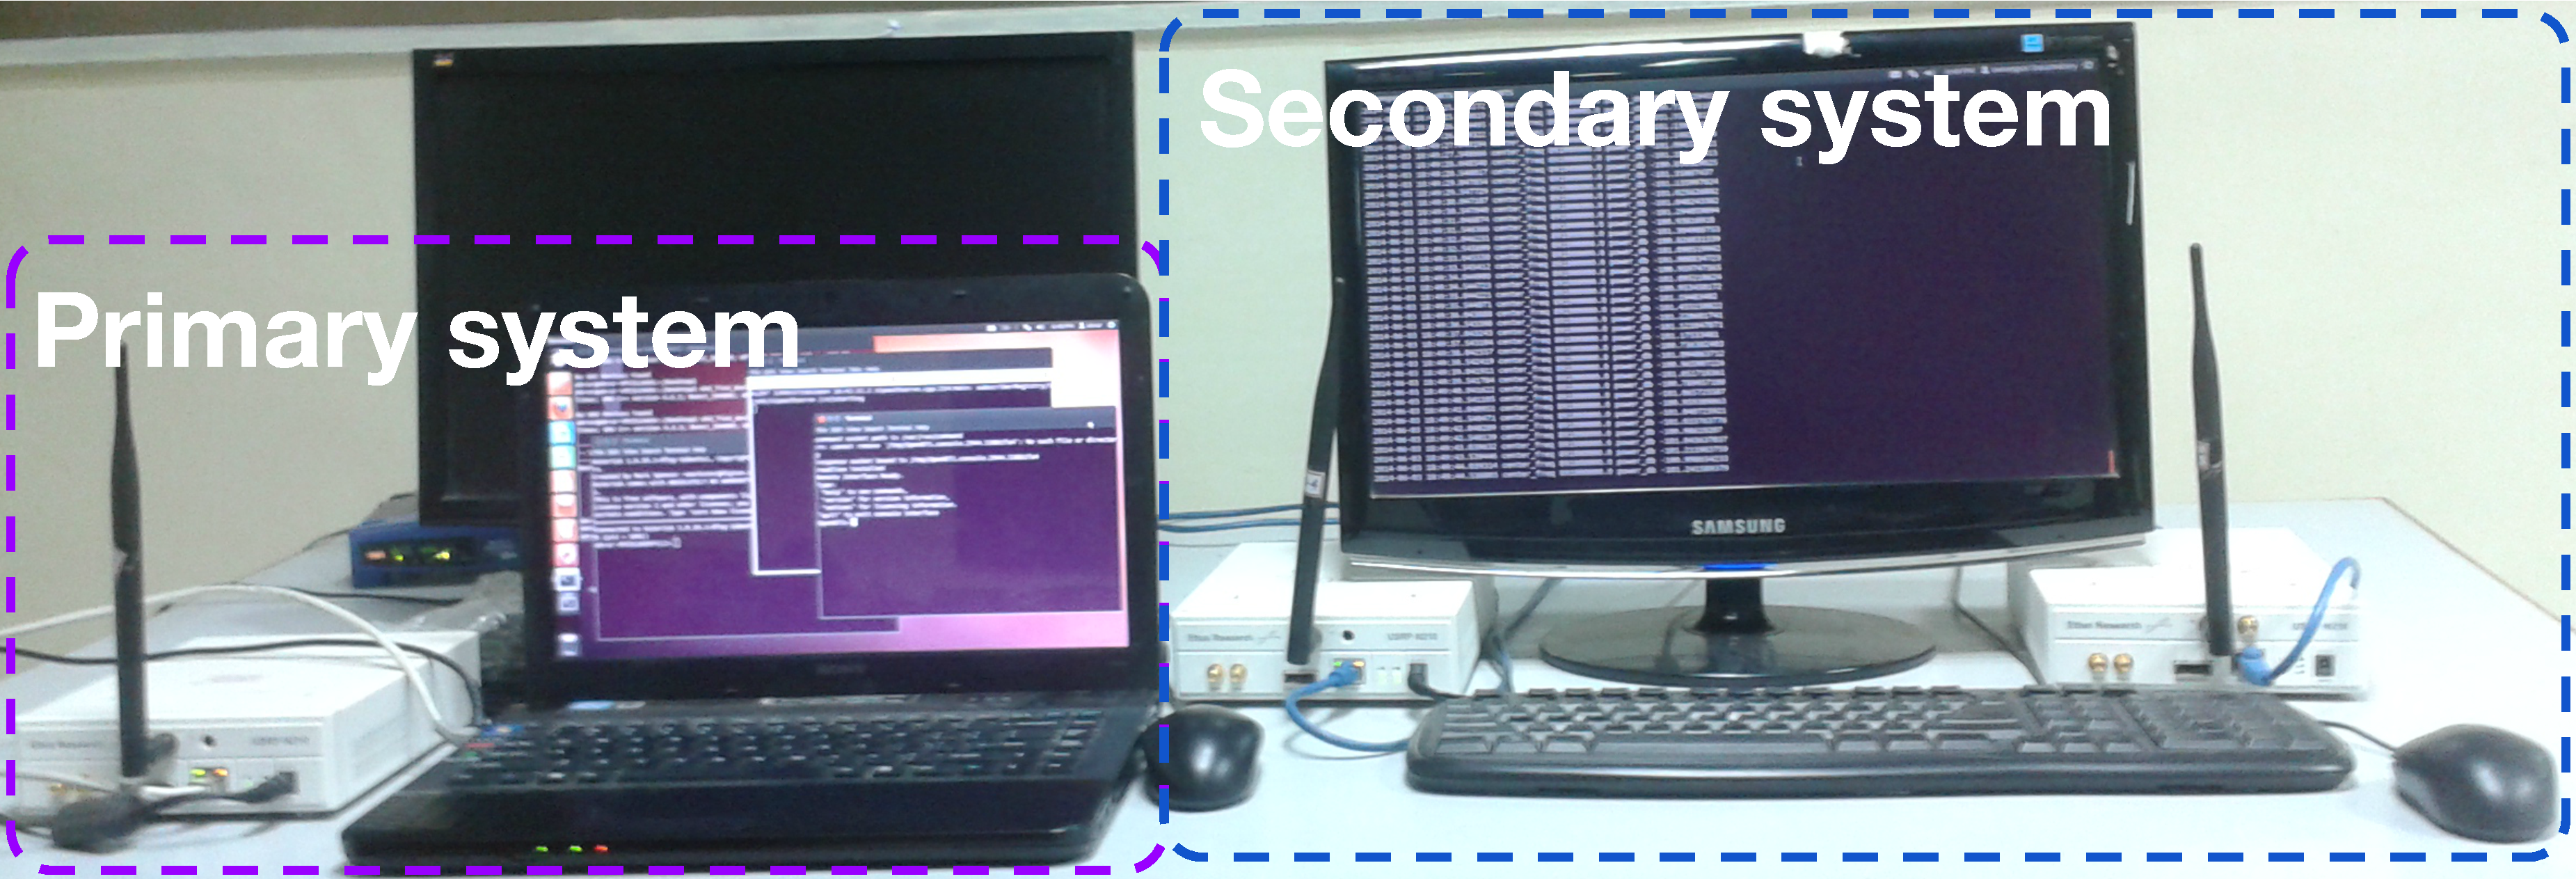
\includegraphics[width=\linewidth]{img/freq2}
    \end{figure}
  \end{frame}
  
  \begin{frame}{Setup for the 4-frequency test-bed}
    \begin{figure}
      \centering
      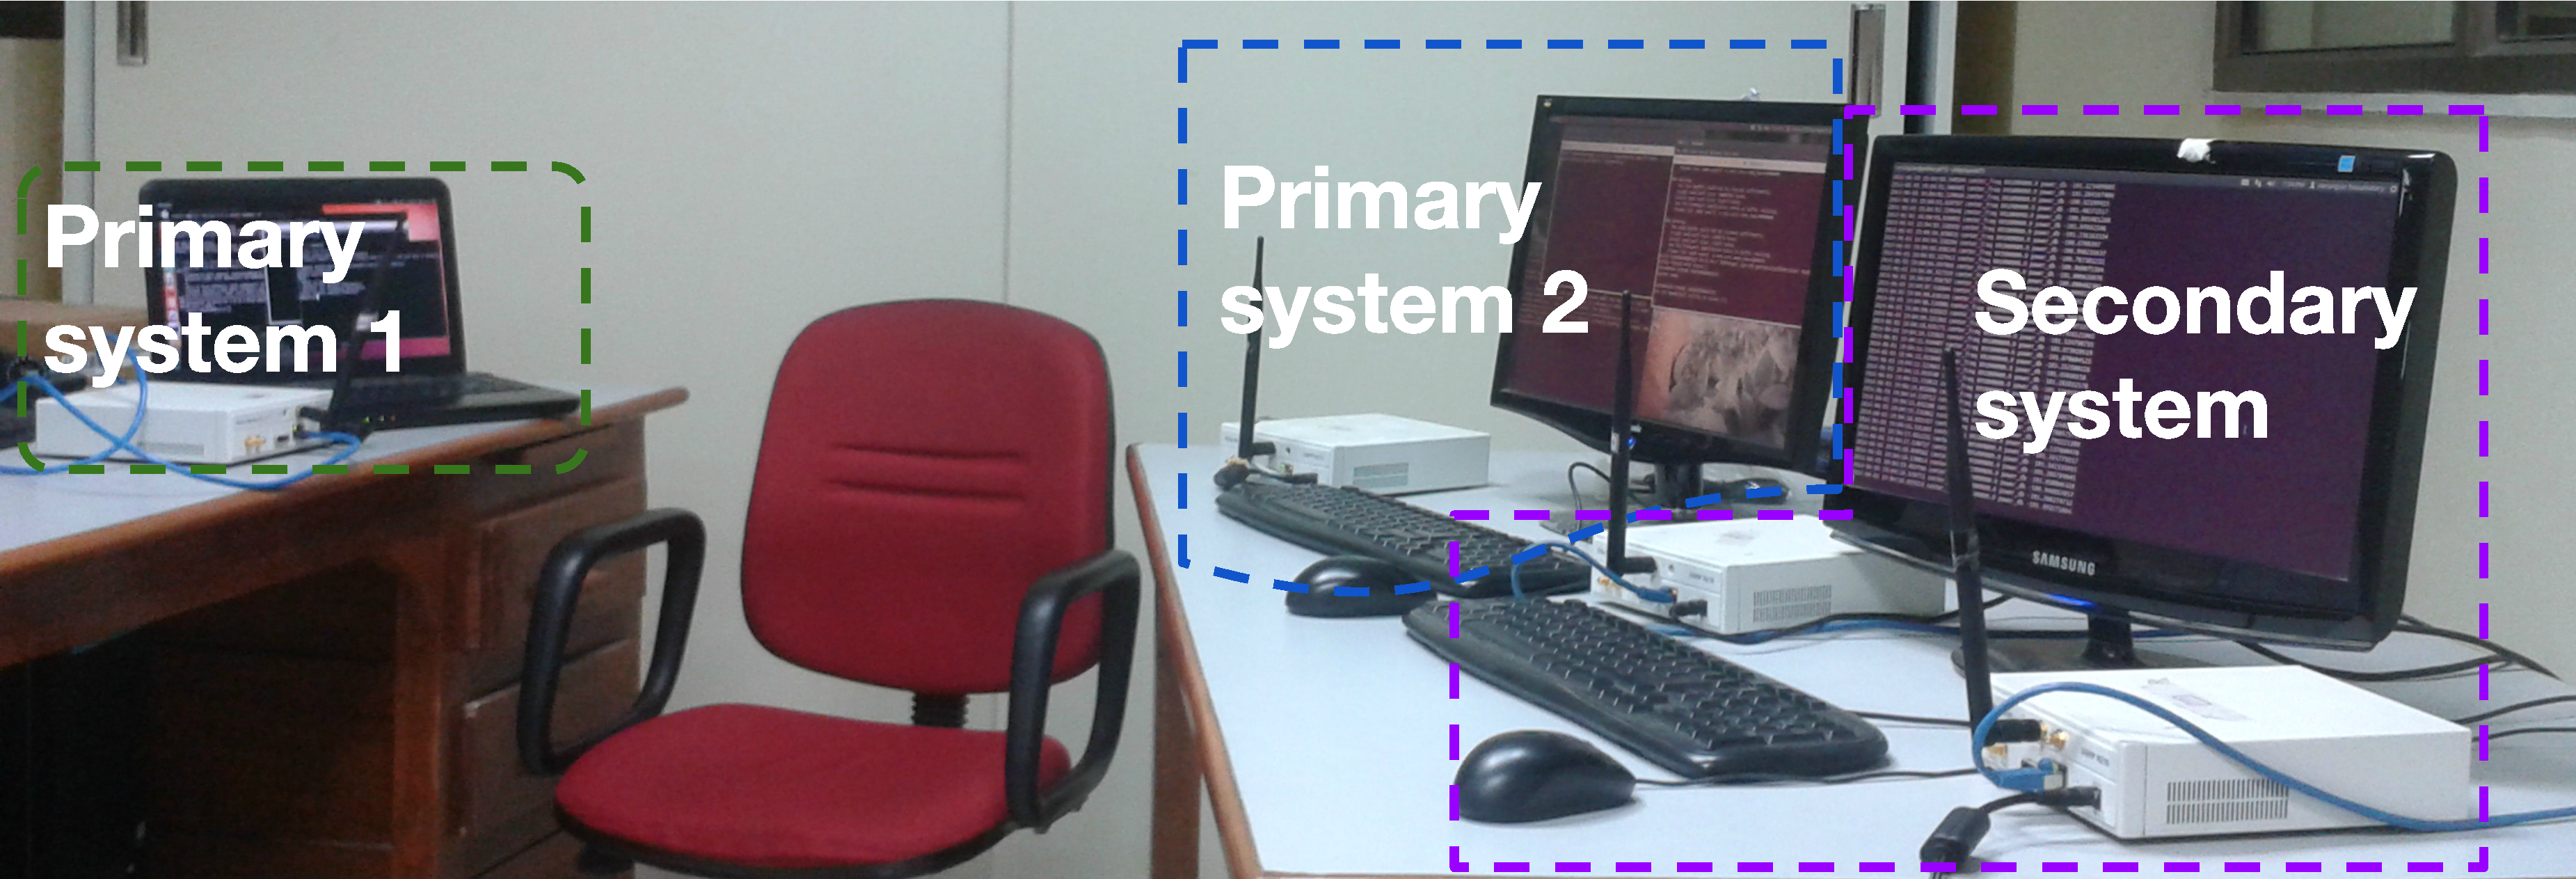
\includegraphics[width=\linewidth]{img/freq4}
    \end{figure}
  \end{frame}
    
  \begin{frame}{Cognitive Radio}
    \begin{minipage}[t][0.8\textheight][t]{\textwidth}
      \begin{itemize}
        \item What is Cognitive Radio?
      \end{itemize}
      \begin{figure}
        \centering
        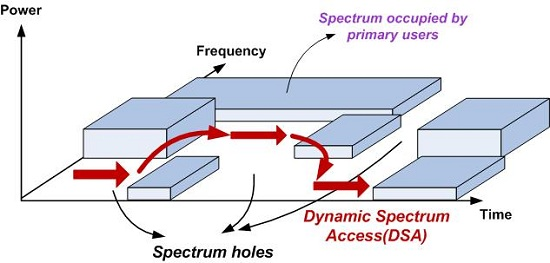
\includegraphics[width=\linewidth]{img/freqUtil}
      \end{figure}
      \vfill
      \tiny{Source: \url{http://www.brunel.ac.uk/\_\_data/assets/image/0011/237539/Abdullah-Masrub1.jpg}}
    \end{minipage}
  \end{frame}

   \begin{frame}{GSM}
    \begin{minipage}[t][0.8\textheight][t]{\textwidth}
      \begin{figure}
        \centering
        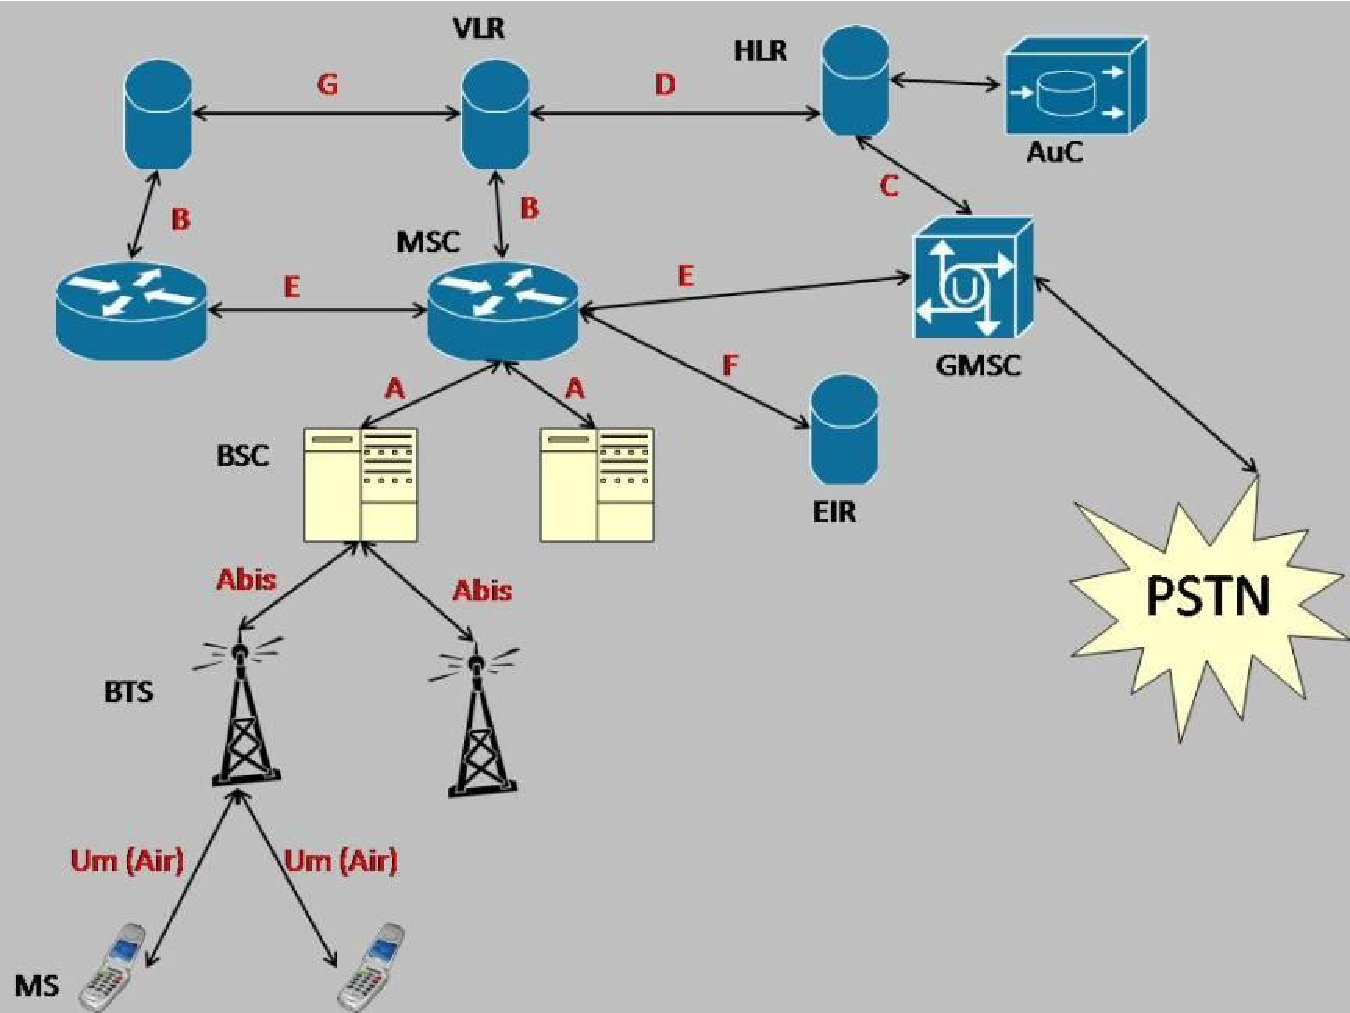
\includegraphics[width=0.8\linewidth]{img/gsmNetwork}
      \end{figure}
      \vfill
      \tiny{Source: \url{http://gnuradio.org/redmine/attachments/download/156/fullnetwork.jpg}}
    \end{minipage}
  \end{frame}
 
  \begin{frame}{Software Defined Radio}
    \begin{itemize}
      \item What is software defined radio?
      \item Block Diagram:
    \end{itemize}
    \begin{figure}
      \centering
      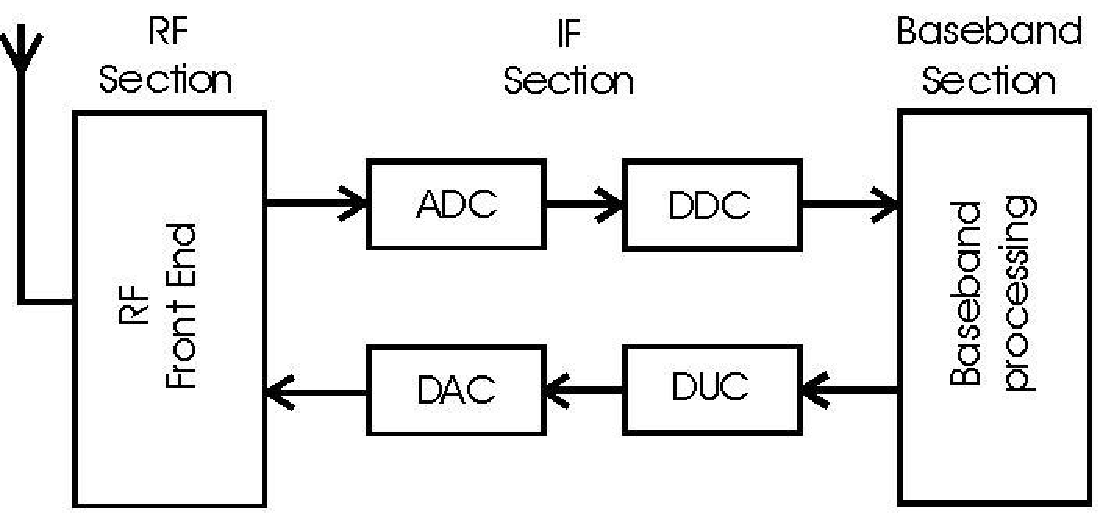
\includegraphics[width=\linewidth]{img/sdrBlock}
    \end{figure}
  \end{frame}

  \begin{frame}{USRP}
    \begin{itemize}
      \item We have used the USRP N210 kit. It performs the task of: transmission, receiving and sensing
      \item The kit is equipped with WBX daughter board which spans a spectrum range of: 50-2200MHz
    \end{itemize}
    \begin{figure}
      \centering
      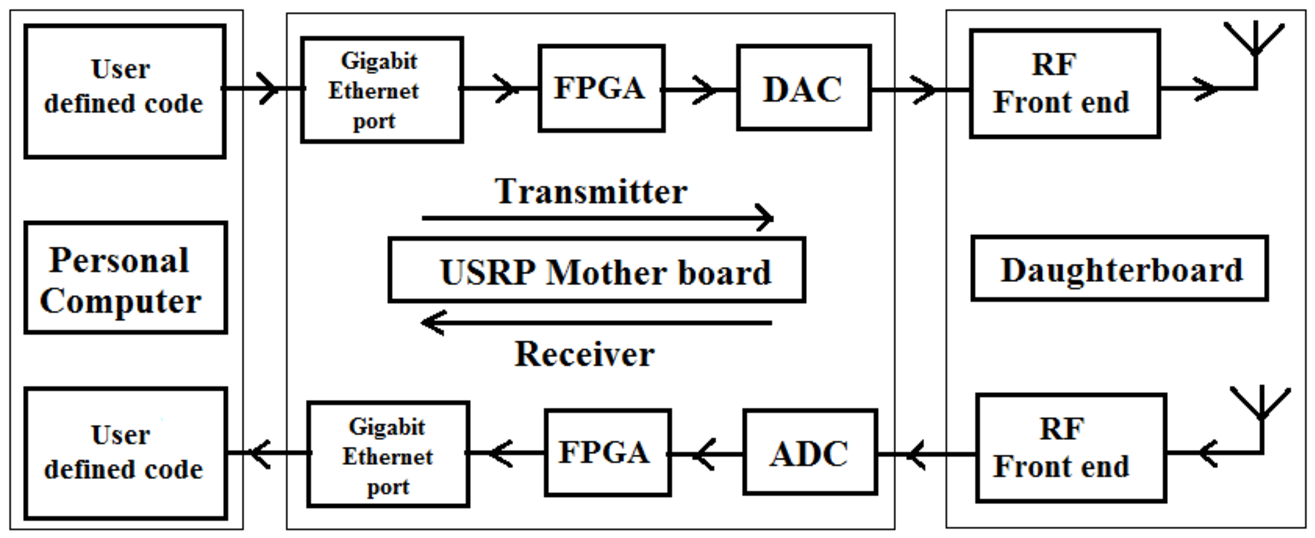
\includegraphics[width=\linewidth]{img/usrpBlock}
    \end{figure}
  \end{frame}
  
  \begin{frame}{GNURadio}
    \begin{itemize}
        \item What is GNU Radio?
        \item Skeleton code spectrumsense.py
        \item Block Diagram
    \end{itemize}
    \begin{figure}
      \centering
      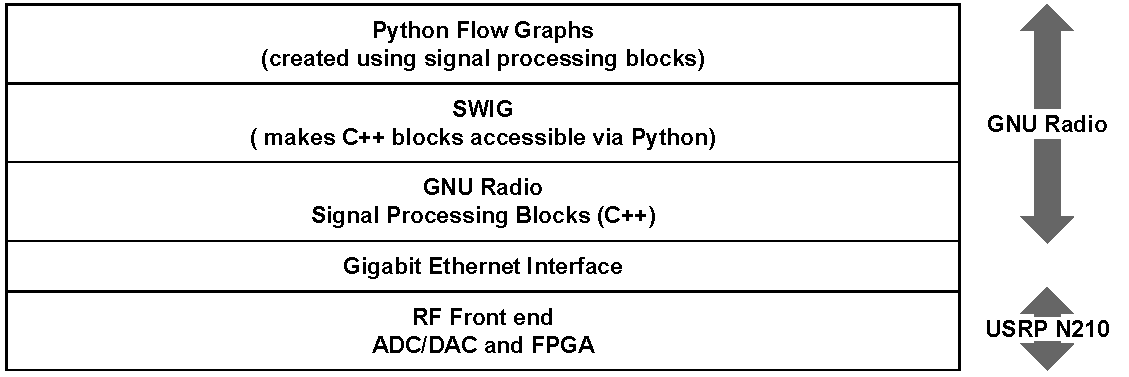
\includegraphics[width=\linewidth]{img/gnuradio_architecture}
    \end{figure}
  \end{frame}

  \begin{frame}{Block diagram of SDR using USRP and GNURadio}
    \begin{figure}
      \centering
      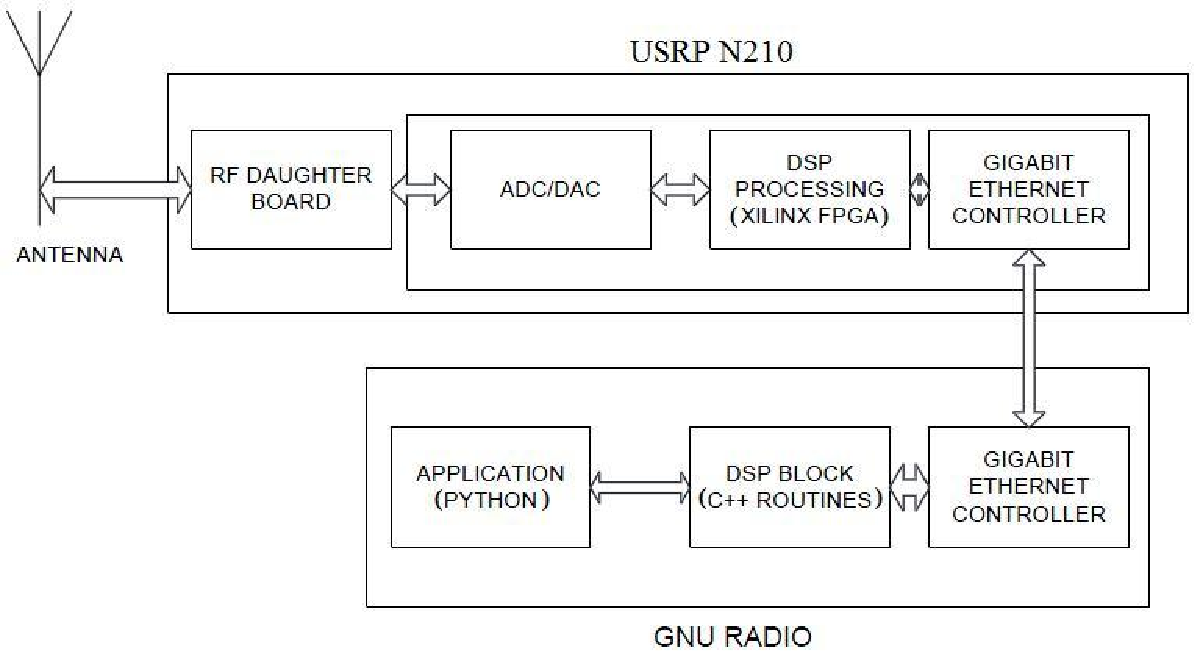
\includegraphics[width=\linewidth]{img/usrpGNURadioBlock}
    \end{figure}
  \end{frame}

  \begin{frame}{OpenBTS}
    \begin{itemize}
      \item Motivation of  building OpenBTS
      \item What is OpenBTS?
      \item The OpenBTS Application Suite
        \begin{itemize}
          \item[-] OpenBTS
          \item[-] Asterisk
          \item[-] Smqueue
          \item[-] SIPAuthServe (Subscriber Registry)
        \end{itemize}
    \end{itemize}
  \end{frame}
  \begin{frame}{Block diagram of SDR using USRP and GNURadio}
    \begin{figure}
      \centering
      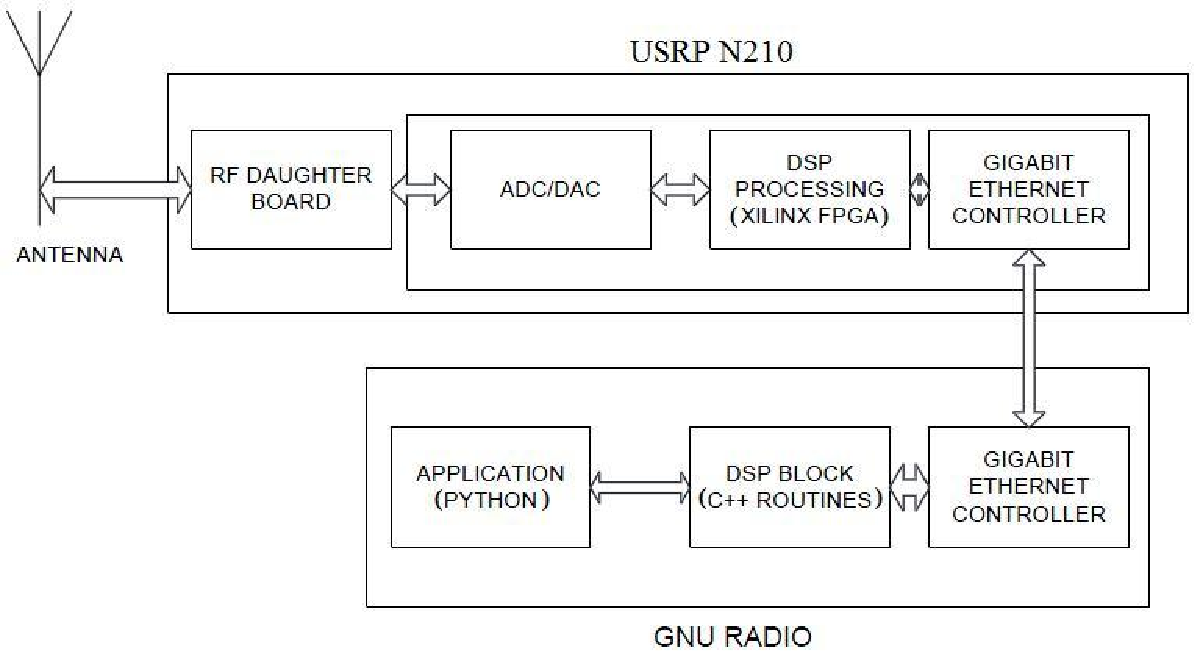
\includegraphics[width=\linewidth]{img/usrpGNURadioBlock}
    \end{figure}
  \end{frame}

  \begin{frame}{How to register a SIM in the network?}
    \begin{itemize}
      \item Sip.conf
      \item Extensions.conf
      \item Sqlite3.db
    \end{itemize}
    \begin{figure}
      \centering
      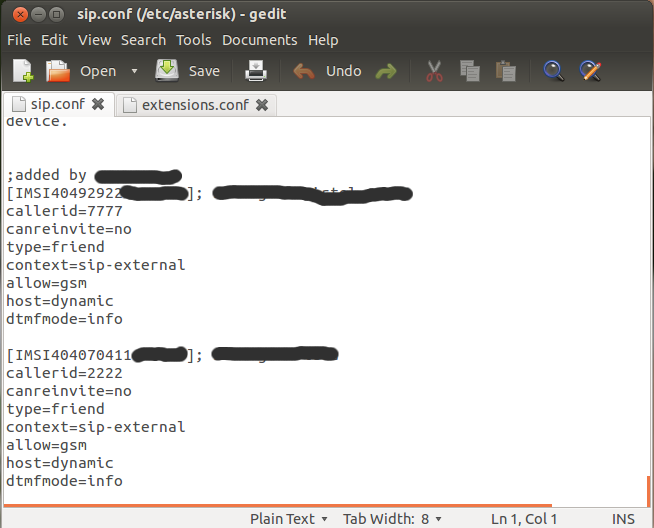
\includegraphics[width=0.7\linewidth]{img/sip_conf}
    \end{figure}
  \end{frame}
  
  \begin{frame}{How to register a SIM in the network?}
    \begin{figure}
      \centering
      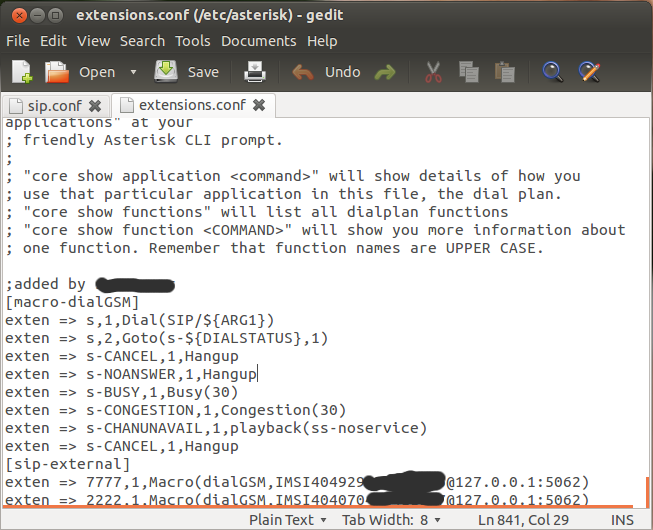
\includegraphics[width=0.7\linewidth]{img/ext_conf}
    \end{figure}
  \end{frame}
  
  \begin{frame}{How to register a SIM in the network?}
    \begin{figure}
      \centering
      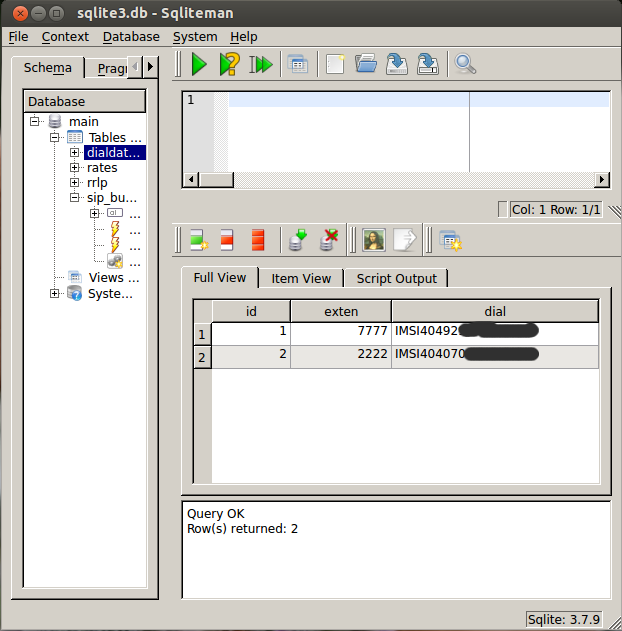
\includegraphics[width=0.7\linewidth]{img/dialdata}
    \end{figure}
  \end{frame}
  
  \begin{frame}{How to register a SIM in the network?}
    \begin{figure}
      \centering
      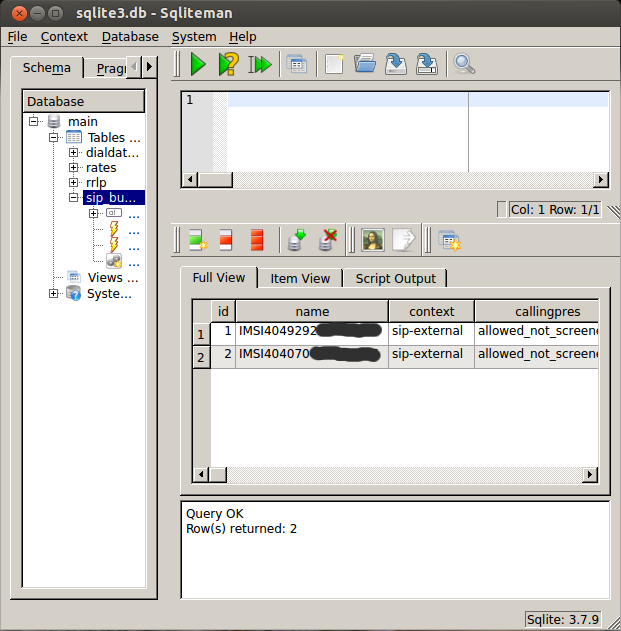
\includegraphics[width=0.7\linewidth]{img/sipbuddies}
    \end{figure}
  \end{frame}

  \begin{frame}{Network organization for OpenBTS}
    \begin{figure}
      \centering
      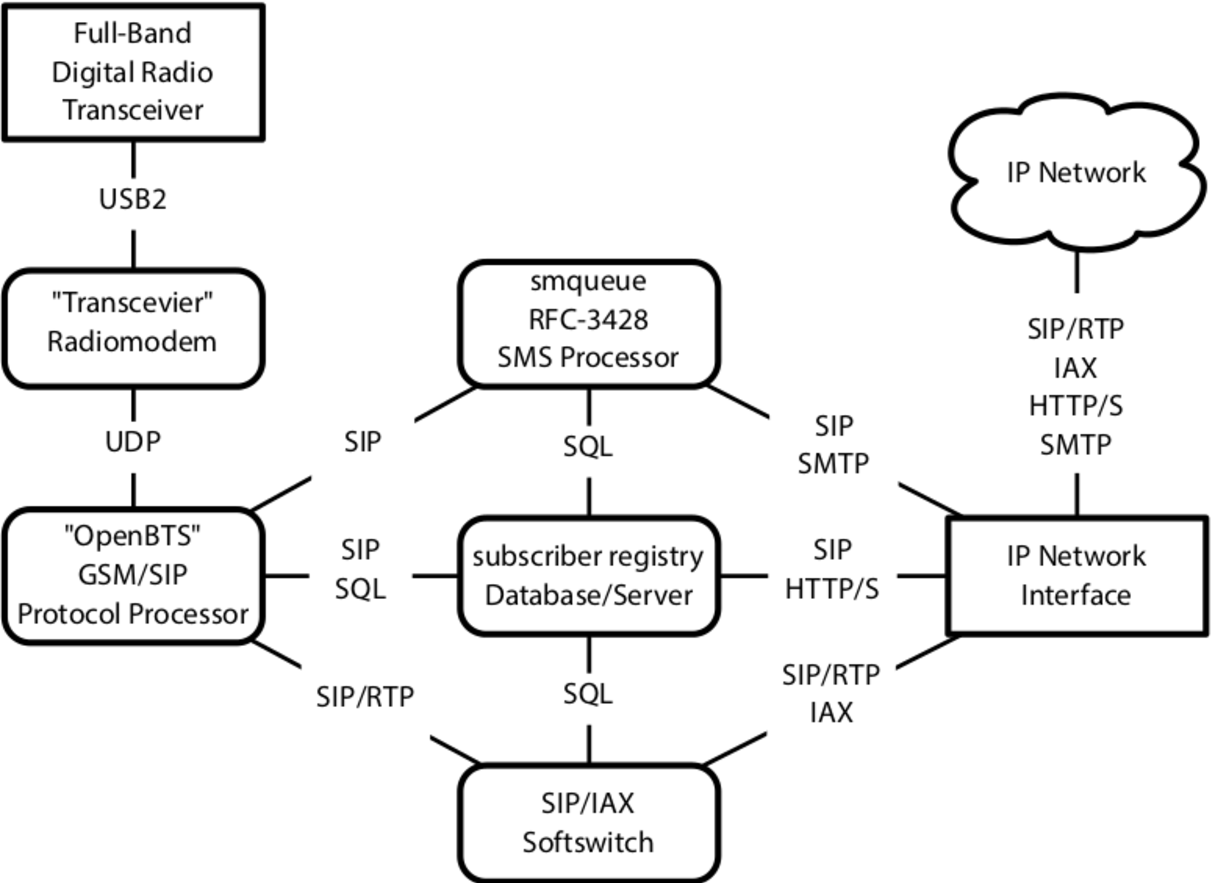
\includegraphics[width=0.97\linewidth]{img/btsSimple}
    \end{figure}
  \end{frame}
  
  \begin{frame}{Spectrum sensing}
    \begin{itemize}
      \item What is spectrum sensing?
      \item Various techniques:
      \begin{enumerate}
        \item Matched filter based technique
        \item Energy detection based technique
      \end{enumerate}
    \end{itemize}
  \end{frame}

  \begin{frame}{Matched filter detection}
    \begin{itemize}
      \item Correlation with a filter whose response is matched with reference signal
      \item Block diagram:
    \end{itemize}
    \begin{figure}
      \centering
      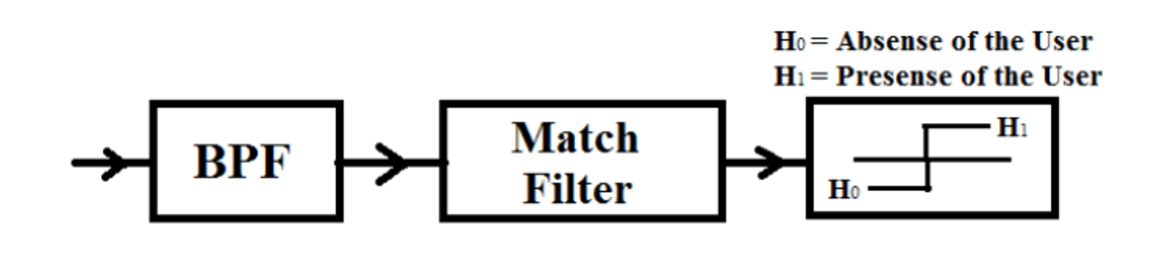
\includegraphics[width=0.97\linewidth]{img/matchedFilter}
    \end{figure}
  \end{frame}

   \begin{frame}{Energy detection technique}
    \begin{minipage}[t][0.8\textheight][t]{\textwidth}
      \begin{itemize}
        \item Hypothesis testing
        \item Equations
          \begin{align}
            x(t) &= n(t), & H_0 \nonumber \\
            x(t) &= h(t)s(t) + n(t), & H_1 \nonumber
          \end{align}
        \item Block diagram
      \end{itemize}
     \begin{figure}
        \centering
        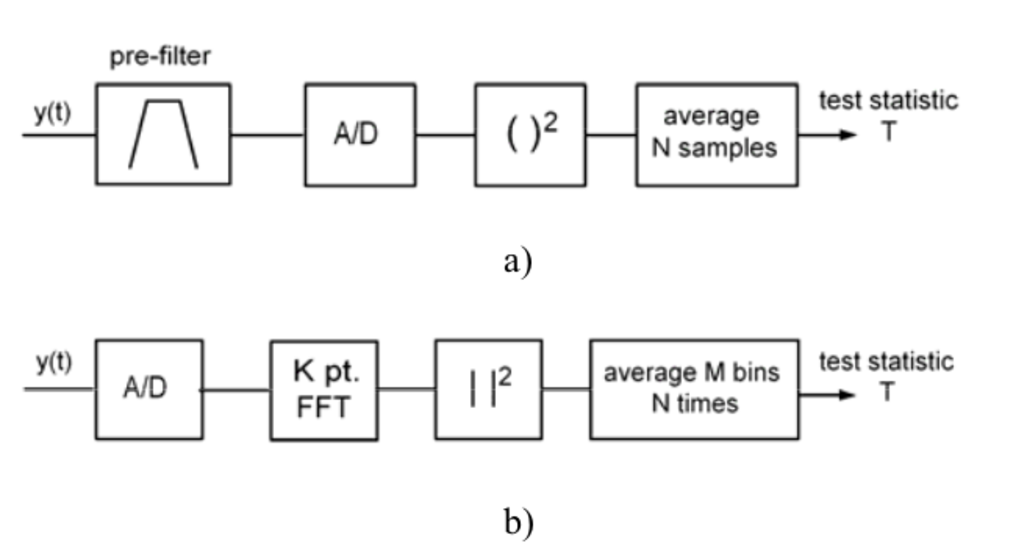
\includegraphics[width=0.8\linewidth]{img/energyDetection}
      \end{figure}
      \vfill
      \tiny{Source: \url{http://www.hindawi.com/journals/ijvt/2011/630467.fig.003.jpg} 
      [Accessed  on Oct 22, 2013.]}
    \end{minipage}
  \end{frame}

  \begin{frame}{Periodogram Analysis}
    \begin{itemize}
        \item $X[n]; n = 0,1...L-1$ is  divided into $M$ finite length 
        segments $X_{r}[n]; n = 0,1...N-1 $
        \item The modified periodogram for the $r$th segment is,
          \begin{equation*}
              I_{r}[k] = \frac{1}{NU} \left| V_{r}[k]\right|^2     \qquad k = 0,1...N-1 
          \end{equation*}
          where $V_{r}[k] = DFT\{W[n]*X[n]\}$, N point DFT
          and $U = \frac{1}{N}(\sum_{n-0}^{N-1} (W[n])^2)$ is the normalization factor. 
        \item The PSD of $X[n]$ sequence 
          is then the time averaged periodogram estimate ,
          \begin{equation*}
              I[k] = \frac{1}{M}\left|\sum_{r=0}^{M-1}X_{r}[k]\right|
          \end{equation*}
    \end{itemize}
  \end{frame}

  
  
  
  
  \begin{frame}{2-frequency system}
    \begin{itemize}
      \item Channels used: 945MHz and 955MHz
      \item Experimental setup :
    \end{itemize}
    \begin{figure}
      \centering
      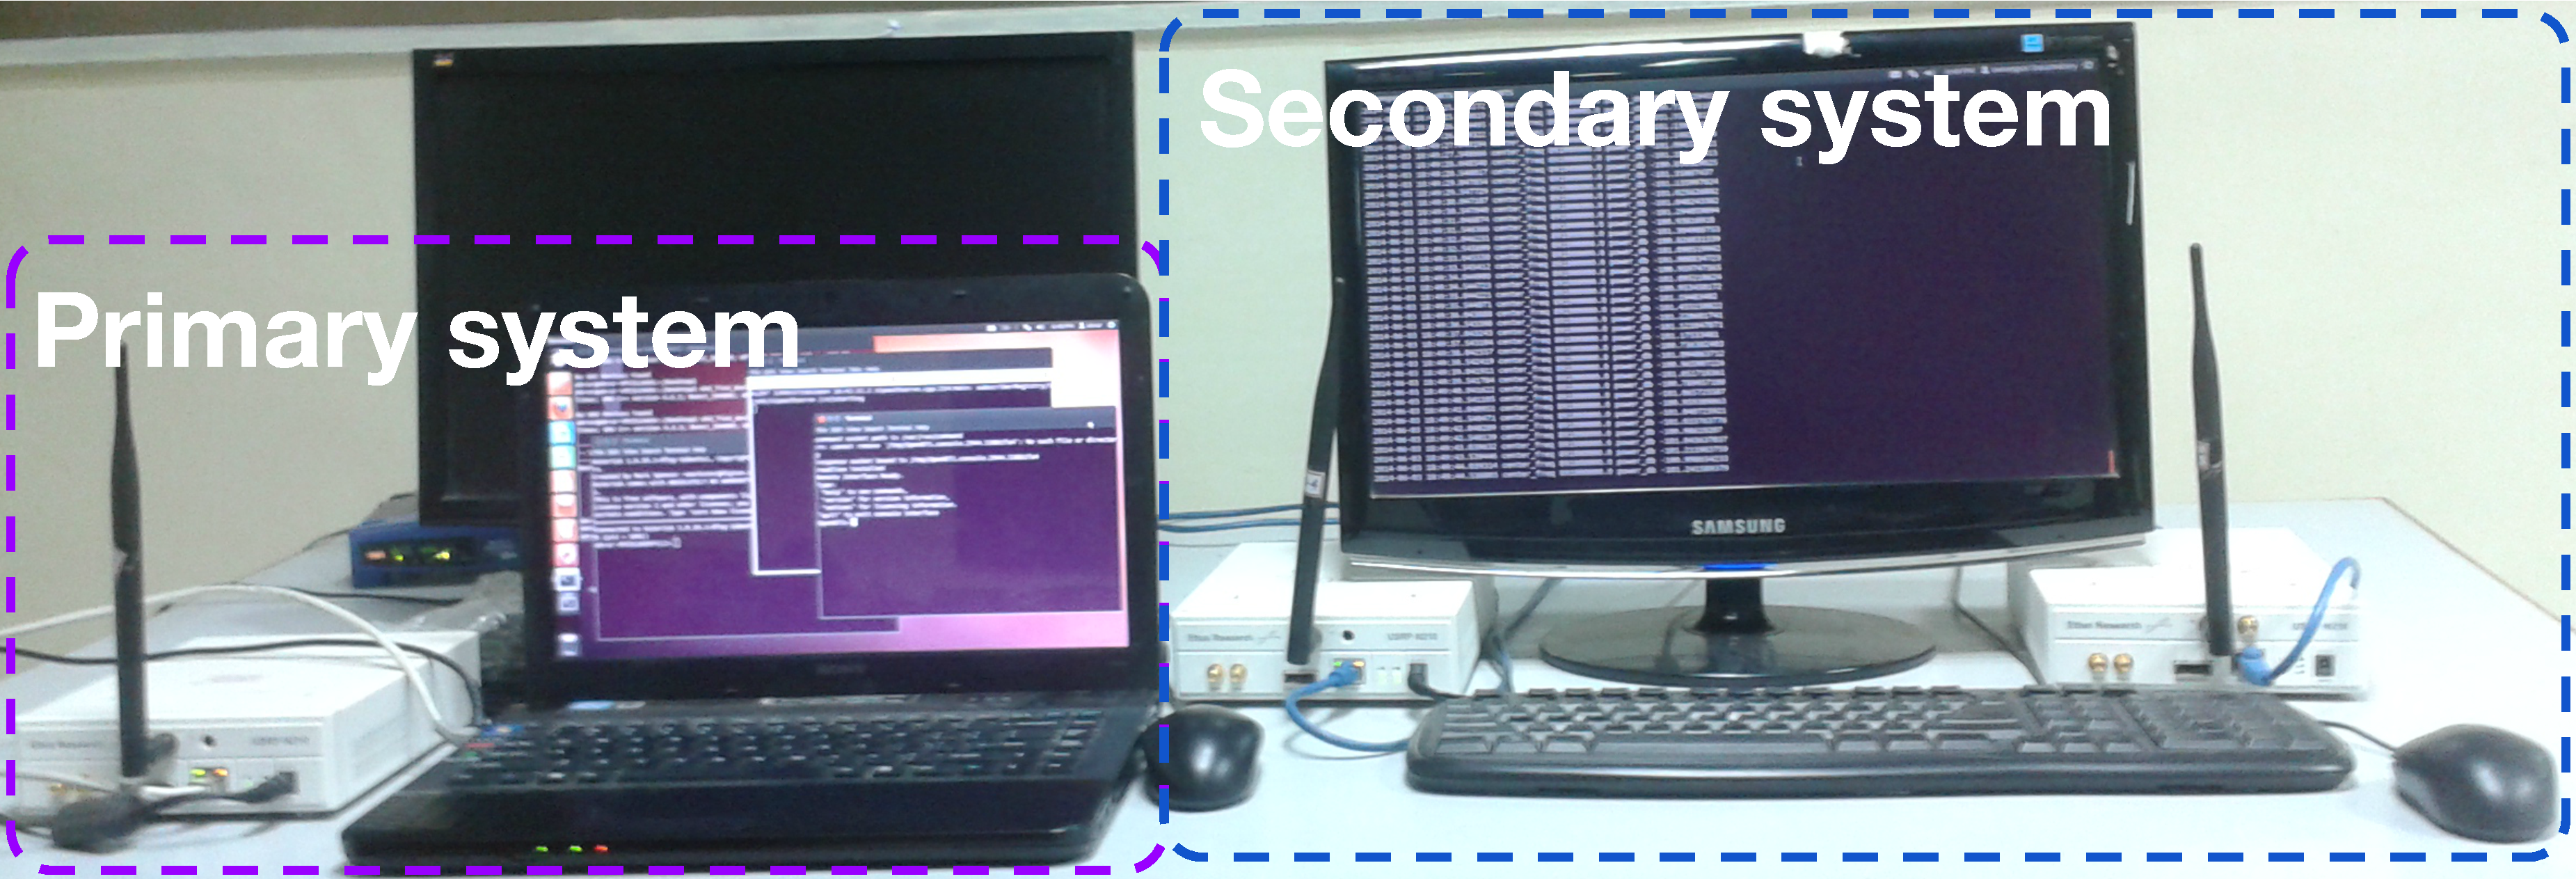
\includegraphics[width=0.97\linewidth]{img/freq2}
    \end{figure}
  \end{frame}
  
  \begin{frame}{Flow chart for 2-frequency system}
    \begin{figure}
      \centering
      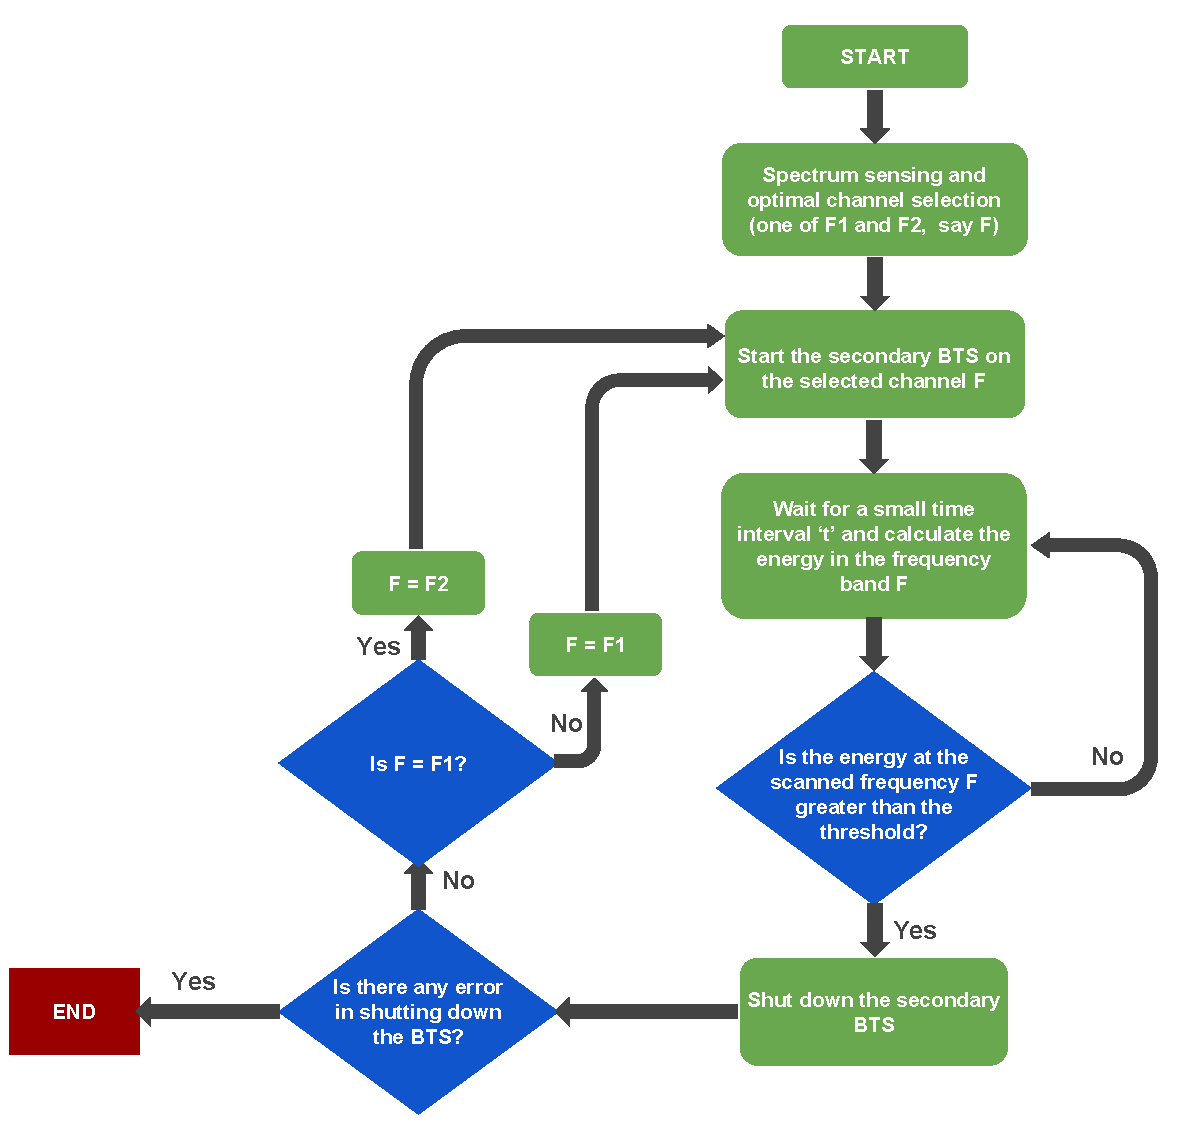
\includegraphics[height=0.9\textheight]{img/freqSys2}
    \end{figure}
  \end{frame}

  \begin{frame}[c]
    \begin{center}
      \LARGE \textbf{VIDEO for 2-frequency system}
    \end{center}
  \end{frame}


  
  \begin{frame}{4-frequency system}
    \begin{itemize}
      \item Channels used: 936MHz, 943MHz , 950MHz , 957MHz
      \item Experimental setup :
    \end{itemize}
    \begin{figure}
      \centering
      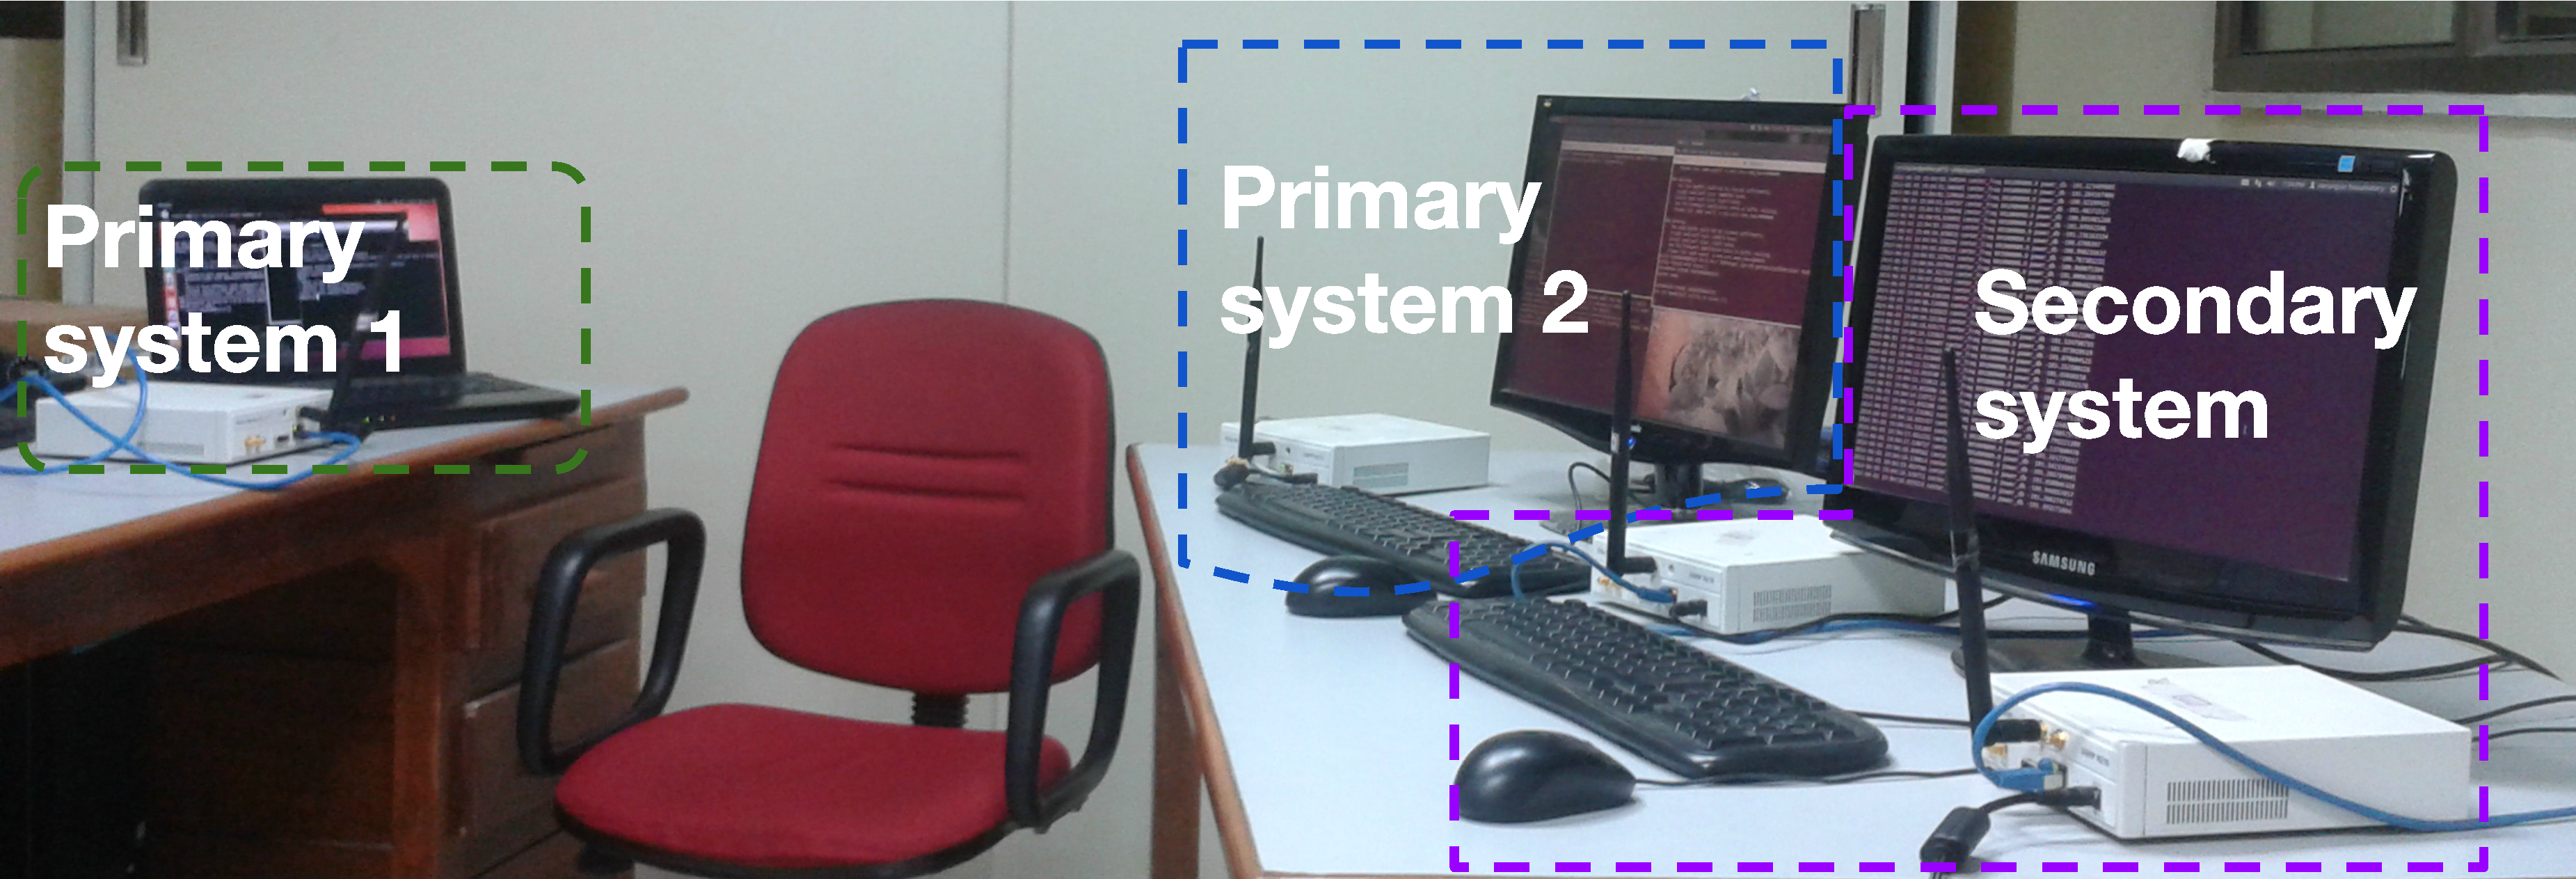
\includegraphics[width=0.97\linewidth]{img/freq4}
    \end{figure}
  \end{frame}
  
  \begin{frame}{Flow chart for 4-frequency system}
    \begin{figure}
      \centering
      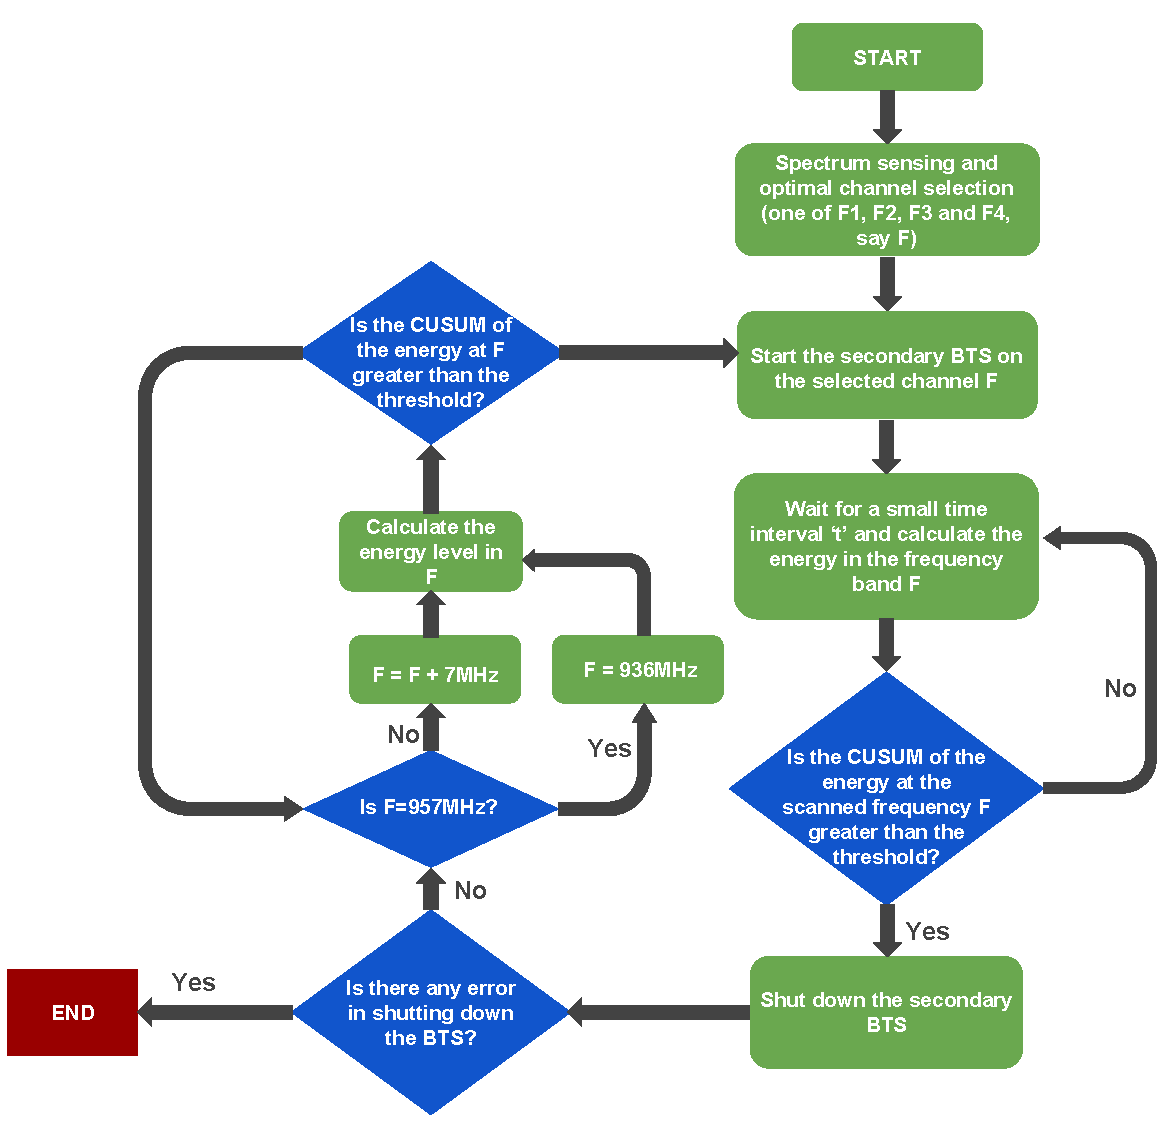
\includegraphics[height=0.9\textheight]{img/freqSys4}
    \end{figure}
  \end{frame}

  \begin{frame}[c]
    \begin{center}
      \LARGE \textbf{VIDEO for 4-frequency system}
    \end{center}
  \end{frame}
    
\end{document}